\cotefile{156-3}
\scanpage{26}\mspage{25}
% L1–4
pour
\[
\partial T=\text{bord absolu de }T
=\left\{\deleted{t\in T\mid t\text{ est }}\begin{aligned}
&\text{un plus petit}\\[-2pt]
&\text{ou plus grand}\\[-2pt]
&\text{élément de }T
\end{aligned}\right\}
\]
% L5–6
\deleted{Si $T$ est réduit à un pt,}

On a donc
% L7–10
\[
\begin{aligned}
\partial\{a\}&=\{a\}\\
\partial[\unsure{o|a|0},b]&=\{a,b\} &&\text{si }a\leq b\\
\partial L_{\geq a}&=\partial L_{\leq a}=\{a\} &&\forall\,a\in L\\
\deleted{\unsure{\partial L=\varnothing}}\quad\partial L&=\partial L\quad\text{(sic)}
\end{aligned}
\]
\margin{(sans exclure le cas $a\in\partial L$)}
% L11–12
Notons que
\[
T^\bullet\cap T\subset\partial T\subset\deleted{\partial L}(T^\bullet\cap T)\cup\partial L
\]
% L13–15
i.e tout $t\in T$ qui est pt frontière, est dans le bord \inserted{de $T$}, et l'inverse est vrai si $t\notin\partial L$. Plus précisément
% L16–18
\[
\begin{aligned}
&\deleted{\text{Si }\operatorname{Card}\,T=1_{\unsure{\mathrm{elt}|\mathrm{él}}},\quad\partial T=T^\bullet=T}\\
&\deleted{\text{Sinon}}\quad
\left\{\begin{aligned}
&\deleted{T^\bullet\cap T=\partial T\setminus(\partial T\cap\partial L)}\quad\deleted{\text{\unsure{i.e.}}}\\
&\deleted{\partial T=(T^\bullet\cap T)\cup T\cap\partial L}
\end{aligned}\right.
\end{aligned}
\]
% L19
\[
\boxed{\partial T=(T^\bullet\cap T)\mathbin{\underline{\cup}}(T\cap\partial L)}
\]
% L20–22
\unsure{Tronçons|Tronçon} : C'est une partie \deleted{\unsure{de la réduite|de la réunion}} \deleted{de la forme} \deleted{\unsure{convexe}} de la forme $T'=T\setminus\alpha$, avec $\alpha\subset\partial T$.

\deleted{\unsure{Tronçon ouvert|Tronçons ouverts} :} c'est un ens de la forme
% L23–26
\[
\left\{\begin{aligned}
&]a,b],\;[a,b[,\;]a,b[,\quad(a<b)\\
&L_{<a},\ \deleted{\unsure{a\in\partial L})}\quad(a\neq\omega)\\
&L_{>a}\hspace{7em}(a\neq\alpha)\\
&L
\end{aligned}\right.
\]
% slanted
% L lower left, oblique
\margin{\uline{NB} Cette écriture est \uline{unique} on pose $T=\widetilde{T'}$ (c'est une \unsure{sorte} d'adhérence \unsure{de $T$|de $T'$} -- \unsure{c'est} le \unsure{sous-tronçon|seul tronçon} le plus petit fermé \unsure{qui contient} $T'$.}
\scanpage{27}\mspage{26}
% L1–5
Les tronçons $]a,b[,\ L_{<a},\ L_{>a},\ \inserted{L}$ sont dits ouverts \deleted{(\uline{NB} ils sont} \deleted{(ce sont bien ceux} \inserted{(ce sont bien ceux qui sont} ouverts pour la top. can.), \deleted{qui sont ouverts} et $]a,b]$ et $[b,\unsure{o|a|0}[$ sont dits \uline{demi}-\uline{ouverts}.

% L6–11
\uline{Attention} \deleted{Le tronçon} Si $a$ plus petit \unsure{élém|élément}, alors $[a,b[$, \deleted{est ouvert} \inserted{qui est} demi-ouvert pour la terminologie précédente, est aussi ouvert pour la top. canonique, et il est égal à $L_{<b}$. Kif kif dualement. $L$ est à la fois ouvert et fermé.

% L12–14
Un \uline{tronçon} \uline{générali\deleted{\unsure{sé}}\unsure{sé}} \inserted{ou ps.tronçon} est une partie de $L$ qui est soit réduit à un pt, soit un tronçon. Pour un tronçon de la forme
% L15–16
\[
\deleted{\unsure{T}}\ T'=T\setminus\alpha\qquad(T\text{ tronçon fermé},\ \alpha\in\partial T
\]
je pose
\[
\partial T'=\partial T
\]
% L17–18
et \unsure{on aura|l'on aura} \unsure{encore|que}
\[
\partial T'=\unsure{T'\mathbin{\dot\cup}|{T'}^\bullet\mathbin{\underline{\cup}}}\partial L\deleted{\unsure{.}}
\]
\margin{Attention, cette fois ce n'est pas le $\partial$ absolu de $T'$ pour la structure d'ordre induite. \unsure{\ldots}}
% slanted
% L lower left, oblique
\margin{\uline{NB} $\partial T'\neq\varnothing$ sauf \unsure{qd|q} si $T'=L$, $L$ \unsure{un|une} \deleted{\unsure{``droite ouverte''}} \deleted{\unsure{ligne}} \unsure{tronçon-interminable}\ldots\ Les pts frontière de $T'$ sont \deleted{ses} bornes inf. et sup. \uline{dans $T$} (si elles existent) : borne sup (ssi $T'$ est majoré) borne inf (ssi $T'$ est minoré) égales \unsure{ds} le cas $T$ \unsure{réduit} à un pt\ldots}

% L19–22
\deleted{\unsure{Soient} deux} Deux ps.tronçons \inserted{$T,T'$} sont dits \uline{en pos. relative modérée} (abrég, $(T,T')$ \deleted{\unsure{en p.}} modéré ou $\{T\unsure{\mid|,}T'\}$ modéré) si $\partial T$ et $\partial T'$ le sont, i.e $\partial T\cup\partial T'$ est tot. ordonné.
\scanpage{28}\mspage{27}
% L1–3
\noindent\llap{\rule[-1.05\baselineskip]{0.4pt}{1.85\baselineskip}\hspace{0.65em}}\uline{Prop} Si $T,T'$ sont des ps. tr. en position rel modérée, alors $T\cap T'$ est \inserted{vide ou est} un ps. tr, et on a
\[
\partial(T\cap T')\subset\partial T\cup\partial T'
\]

% L4–6
Immédiat. On va introduire une relation d'ordre entre ps-tronçons \inserted{(pas l'inclusion!)}. On dit que
\[
T\unsure{<|\prec}T'
\]
% L7–8
si \deleted{a) $T$ est en pos. rel modérée avec $T'$,}
\[
\deleted{\text{b)}}\quad\deleted{\unsure{\forall}}\quad t\in T,\ t'\in T'\implies t<t'
\]
\margin{\leavevmode\llap{\rule[-4\baselineskip]{0.35pt}{5\baselineskip}\hspace{0.4em}}\deleted{\unsure{Si les}} Ça implique $T$ et $T'$ en pos. rel. mod et $T\cap T'=\varnothing$}
% L9
C'est \unsure{évident|évidemt} transitif.

% L10–15
Soit $T<T'$. Comme $T$ est majoré, il s'ensuit que \deleted{$\partial T\neq\varnothing$} il a un plus grand \unsure{élém|élément} \deleted{\unsure{b}} $a$, \deleted{tel que} \inserted{et alors} $T\subset L_{\leq a}$. \deleted{\unsure{Comme}} De $=$, $\partial T'$ a un plus petit élément $b$, tel que $T'\subset L_{\geq b}$, \deleted{\unsure{et on a}} \deleted{\unsure{alors}} et on voit de suite que $a\leq b$.

% L16 and note below brace
\uline{Position relative \deleted{impropre} \inserted{de raccordement}} : $a=b$, et $\underbrace{a\in T\text{ ou }b\in T'}$%
\margin{à l'exclusion l'un de l'autre, puisque $T\cap T'=\varnothing$}

% L17–20
\deleted{\unsure{Pour|Par} la suite, on l'\uline{exclut} \unsure{donc} :}

On renforce la relation $<$ en $\ll$
\[
\begin{aligned}
T\ll T' &\Longleftrightarrow T<T',\quad\text{et position relative}\\
&\hspace{12em}\text{propre}\\
&\Longleftrightarrow \exists\,x\in L\text{ tel que }T\subset L_{\unsure{<|\leq}a},\ T'\subset L_{>x}
\end{aligned}
\]
\scanpage{29}\mspage{28}
% L1
\uline{psTronçon} \uline{interstitiel}

% L2–3
\uline{Prop} Soit $T,T'$ \deleted{ps. tr. tels que $T<T'$}, \deleted{$a=\operatorname{Sup}T,\ b=\operatorname{Inf}T'$}, Conditions équivalentes \deleted{si $a\in{}$} \inserted{(si $a=\operatorname{Sup}T,\ b=\operatorname{Inf}T'$)}

% L4–5
a) $T\unsure{<|\prec}T'$ \inserted{et $T,T'$} ne se raccordent pas, i.e.
\[
(a\in T\text{ ou }b\in T')\implies a\neq b
\]
% L6
\deleted{b) $\exists\,x\in L$}\quad b) $\exists\,x\in L$ tel que $T\subset L_{<\unsure{x|a}},\ T'\subset L_{>\unsure{x|a}}$
% slanted
\margin{\uline{NB} b) implique déjà que $T<T'$}

% L7–9
\deleted{\unsure{b|6}}\unsure{c)|b)} $\exists$ ps. tr. $\deleted{\unsure{I}}S$ tel que
\[
T<\deleted{I}S<T'
\]
et tel que $T$ et $\deleted{I}S$, $\deleted{I}S$ et $T'$ \uline{se raccordent}.

% L10–12
De plus, ce\deleted{\unsure{t}} $\deleted{I}S$ est unique, et $\partial S=\{a,b\}$. $S$ est formé des $x\in L$ tels que
\[
T\subset L_{<a},\ T'\subset L_{>x}\qquad\text{(cf b) )}
\]

% L13–14
On appelle $S$ le ps. tr. interstitiel entre $T$ et $T'$

% L15–19
\uline{Cor} 1 Soit $T$ un tronçon, et supposons que $T$ soit minoré \inserted{\unsure{strictemt|strictement}}. Alors l'ens des \inserted{minorants} \inserted{stricts, i.e. des} $x\in L$ tels que $\unsure{\overline T|T}\subset L_{>x}$ (ens des minorants stricts) est un \deleted{tronçon} ps. tr. $S$, \deleted{que} \inserted{qui satisfait}
% L20
\begingroup
\makeatletter
\tagsleft@true
\makeatother
\[
S<T,\ S\text{ et }T\text{ se raccordent},\ S\text{ sans minorant}\tag*{\(\ast\))}
\]
\endgroup
% L21
et ces conditions \deleted{satisf} caractérisent $S$.

% L22–24
\deleted{\uline{Cor} 2 \unsure{Énoncé|Enoncé} \unsure{de|d}} On appelle $S$ le \uline{pstronçon interstitiel gauche} de \deleted{\unsure{$S$}}$T$, On définit de $=$ (si $T$ majoré) le pstr. interst. droit. de $T$.
\scanpage{30}\mspage{29}
% L1–3
\deleted{\uline{Définition}}

Soit $\operatorname{Tr}(L)$ l'ens \deleted{ordonné} des ps. tronçons de $L$, ordonné par $\ll$.

% L4–6
Pour toute partie finie tot. ordonnée $\Phi$ de $\operatorname{Tr}(L)$, considérons
\[
\deleted{U}X_{\Phi}=\bigcup_{i\in\Phi}T_i\qquad\text{(NB réunion disjointe)}
\]
% L7–12
% slanted
\margin{\uline{Prop}}
Alors l'application
\diagram{\begin{tikzcd}[ampersand replacement=\&,column sep=large,row sep=1.3ex]
\Phi \arrow[r,mapsto] \& \deleted{U}X_{\Phi}\\
\underset{\substack{\text{drapeaux de}\\\operatorname{Tr}(L),\ \text{y inclus}\\\text{\unsure{par|pour|pav|pau}}}}
{\underline{{\operatorname{Drap}}_{\ll}^{\unsure{\partial|b|*|\varnothing}}(\operatorname{Tr}(L))}}
\arrow[r] \& \unsure{\mathcal P|\mathscr P|\mathrm P}(L)
\end{tikzcd}}
est \uline{injective}.

% L13–15
Les ens de la forme $U_{\Phi}$ s'appellent \uline{modérés}. Pour un tel
\[
\deleted{U}X_{\Phi}=\bigcup T_i
\]
on pose
% L16–17
\[
\operatorname{Fr}(\deleted{U}X_{\Phi})=
\underbrace{\left(\bigcup_i\partial T_i\right)}_{\substack{\deleted{\text{\unsure{est}}}\\\partial U,\ \text{drapeau de } L}}\setminus\varepsilon
\]
% slanted
\margin{``frontière'' relative dans $L$ (mais pas pour la topologie \unsure{de|sur} \unsure{m.|sur} $L$\ldots)}
% L18–24
où
\[
\begin{aligned}
\varepsilon={}&\bigl\{t\in\partial L\cap U\mid
  \deleted{\unsure{t\in U}}\ \{t\}\notin\Phi\quad\text{i.e. }\deleted{\unsure{\Phi|\notin}}\\
&\hspace{6em}\{t\}\text{ n'est pas parmi les }T_i,\\
&\hspace{6em}\deleted{\text{i.e. }\exists\,x\in L,\ \text{\unsure{tq} } x<{}}\\
&\hspace{6em}\deleted{\text{i.e. il y}}\quad\text{i.e }U\text{ est un}\\
&\hspace{8em}\text{voisinage de }t\text{ dans } L\\
&\hspace{6em}\text{i.e. }\{t\}\text{ pas point isolé}\\
&\hspace{9em}\text{de }U\ \ldots\bigr\}
\end{aligned}
\]
% slanted
% L lower left note
\margin{Les $T_i$ s'appellent les ``composantes (connexes!) de \deleted{\unsure{$U$}}$X$ (mais pas pour la top canonique) \unsure{l'on|l'ens} \unsure{va|en} \unsure{aussi|sera} \unsure{les|se} \unsure{noter|noté} parfois $\Pi_{\unsure{0|o}}(X)$}
\scanpage{31}
\mspage{30}

% L1–5
\deleted{Ainsi} Soit $\deleted{U}X=\deleted{U}X_{\Phi}$ une partie modérée. Un $x\in L$ est dit en pos. rel. modérée avec $\deleted{U}X$, s'il l'est avec les $T_i$ (\inserted{\uline{tronçons}} \uline{composants} de $\deleted{U}X$) i.e. s'il l'est avec $\underset{\partial U}{\underline{\bigcup\partial T_i}}$, ou encore avec $\operatorname{Fr}(\deleted{U}X)$.
% Lleft margin, alongside lines 1–13
% slanted
\margin{Plus \unsure{généralemt|généralement}, Si $\deleted{U}X\unsure{,|\cap}\deleted{\unsure{V|U'}}Y$ sont modérées, on dit que $\deleted{U}X,Y$ sont en pos. rel. modérée si \deleted{$\partial U$ et $U'$}, $\partial\deleted{U}X,\partial\deleted{V}Y$ le sont ou encore $\operatorname{Fr}\deleted{U}X,\operatorname{Fr}Y$ le sont. Ex: si $\deleted{U}X\subset Y$, alors $(\deleted{U}X,\deleted{V}Y)$ \deleted{\unsure{est}} \unsure{modérée|modéré}.}
% L5–7
Par exemple \deleted{Soit} $x\in\deleted{U}X$, ou $x\in\deleted{\unsure{\operatorname{Fr}|\partial}}\partial U$, à fortiori de $\operatorname{Fr}(\deleted{U}X)$, a cette propriété. Soit
% L8–9
\[
\begin{aligned}
\deleted{U}X'=C_{\mathrm{mod}}\unsure{U U)|(U)|U)}=\bigl\{x\in L\setminus U\mid{}&x\text{ est en pos. rel. mod.}\\
&\text{p.r. à }U\bigr\}
\end{aligned}
\]
% L10–13
Alors \deleted{\unsure{$\mathcal E$|$\mathcal C$|$C$}} $\deleted{U}X'$ est \unsure{modérée|modéré}, et c'est la plus grande partie modérée $\deleted{V}Y$ de $L$ telle que $\deleted{V}Y\subset L\setminus\deleted{U}X$, et $Y$ en position relative modérée par. à $X$. Si
% L14
\[
\{T_1\ll T_2<\ldots\ll T_n\}
\]
% L15–20
est le drapeau définissant \deleted{\unsure{$T$|$\Phi$}} $X$, $X'$ est défini par le drapeau formé des $n-1$ tronçons interstitiels \deleted{entre} pour $(T_1,T_2)$, $(T_2,T_3)$ \ldots\ $(T_{n-1},T_n)$, plus (dans la mesure où ils existent) les tronçons, interstitiel gauche de $T_1$, et le tronçon interstitiel droit du $n$. \unsure{Suite|D'autre}
\scanpage{32}
\mspage{31}

% L1–2
Si $n'$ est le cardinal du $ {\Phi}'\in\operatorname{Drap}_{\ll}^{\unsure{\partial|\alpha|b|*}}(\operatorname{Tr}(L))$ qui définit $X'$, on aura
% L3
\[
n'\in\{n-1,n,n+1\}
\]
% L4–5
donc
\[
\lvert\operatorname{Card}\Pi_{\unsure{0|o}}(X)-\operatorname{Card}\Pi_0(X')\rvert\leq 1
\]
% L6–9
De façon précise
\[\begin{array}{ll}
T_1\ \text{non \unsure{majoré|mijoré}},\ T_n\ \text{non majoré} &: n'=n-1\\
T_1\ \text{minoré et }T_n\ \text{non majoré, ou l'inverse} &: n'=n\\
T_1\ \text{minoré et }T_n\ \text{majoré} &: n'=n+1
\end{array}\]

% L10–12
On considère l'ens \deleted{ordonné} \deleted{(\unsure{cf. ci-dessous|cf. ci-dessus|p. ci-dessus})} des parties modérées de $L$, $\mathcal M=\operatorname{Mod}(L)$. Il y a des structures remarquables

% L13
a) Ordre \quad $X\subset Y$

% L14
b) Relation : $\{X,Y\}$ modérée \quad (NB $\unsure{x|X}\subset Y\Rightarrow\{X,Y\}$ modéré)
% Lleft of b–c
% slanted
\margin{Cette relation est-elle déductible de la relation d'ordre -- p.ex. $\{X,Y\}$ mod ssi $X\wedge Y$ existe ???}

% L15–18
c) Partie $\inserted{\mathcal M_f=}\operatorname{Mod}\mathrm{fer}(L)$ formée des parties modérées dites ``fermées'' (i.e. $X=X_{\Phi}$, où les $T_i$ $(i\in\Phi)$ sont des ps. tr. fermés.)

% L19
\uline{Propriétés}
\scanpage{33}
\mspage{32}

% L1–2
1) Pour la relation d'ordre, il y a un plus petit élément $\varnothing$, et un plus grand élément $L$ \inserted{(ou $1$)}.

% L3
2) : $X\subset Y\Rightarrow\{X,Y\}$ modéré

% L4
3) Si $\{X,Y\}$ modéré, $X\wedge Y$ et $X\vee Y$ existent (inf et sup)
% Lleft, opposite 3
% slanted
\margin{- Attention $X\vee Y$ \deleted{\unsure{est|n'}} n'est \uline{pas} l'union \deleted{de} $X\cup Y$ !!}

% L5–6
\deleted{\unsure{3)|3 bis)} Si $\{X,\unsure{Y_i|Y}\}$ \unsure{est|sont} \illegible{2} modérés, alors} \deleted{Si \unsure{deux|les} $X$ \unsure{et|sont} \unsure{modérés} \unsure{pour}} \inserted{(distributivité) et pour une famille d'\unsure{élmt|élémt} mut\textsuperscript{t} mod, $X\wedge(\bigvee_iY_i)=\bigvee_i(X\wedge Y_i)$}

% L7–11
\deleted{\unsure{3|5}}4) \deleted{Parmi les} $\forall X\in\mathcal M$ \deleted{\unsure{éléments|il existe}}, \deleted{\unsure{dans|du}} parmi les $Y\in\mathcal M$ tels que $\{X,Y\}$ modéré, et $X\wedge Y=\varnothing$, il y a un plus grand élément \inserted{$X'$}. C'est aussi l'unique élément tel que
% Lleft, opposite X′ and tel que
% slanted
\margin{\uline{Dire aussi} Si \deleted{\unsure{(élémt)|($X_i$)}} $\{X_i\}_{i\in\unsure{I|J}}\subset\mathcal M$ est formé d'él\textsuperscript{ts} \unsure{mutuellemt|mutuellement} modérés, alors pour les op. $\wedge,\vee,'$ ils engendrent une ``alg. de Boole'', finie si $I$ fini.\figure{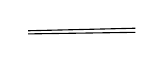
\begin{tikzpicture}[x=.4cm,y=.4cm]\draw (0,0)--(3.4,.08);\draw (0,-.1)--(3.4,-.05);\end{tikzpicture}}}
% L12
\[
\{X',X\}\text{ modéré},\qquad \unsure{X''|X'}\wedge X=\varnothing,\qquad X'\vee X=1
\]
% L13–17
Donc l'application $X\mapsto X'$ est involutive, elle renverse la relation d'ordre (anti-involution), \deleted{donc échange} \deleted{\unsure{De|On}}De plus $\{X\ \mathrm{et}\ Y\}$ sont mod. ssi $\{X',Y'\}$ modéré\textsuperscript{*},
% Lleft of same passage
% slanted
\margin{* En fait, $\forall X,Y$ $\{X,Y\}$ mod. ssi $\{X,Y'\}$ mod (donc ssi $\{X',Y'\}$ mod., \unsure{ssi|et} $\{X',Y\}$ modéré)}
% L18
et alors \quad $(X\wedge Y)'=X'\cup Y'$, \quad $(X\cup Y)'=X'\wedge Y'$

% L19
\deleted{\unsure{4|5}}5) $\varnothing,1\in\mathcal M_f$

% L20–21
\deleted{5}6) $\forall X\in\mathcal M$, il existe un plus petit \deleted{\unsure{4')|$X$|$Y$}} $Y\in\mathcal M_f$ tel que $X\subset Y$ (on pose $Y=\bar X$).
% Lbottom left beside 6
% slanted
\margin{Par passage au compl., on définit $\deleted{\unsure{U|V}}X^{\unsure{\circ|o}}=(\overline{X'})'$.}

% L22–23
De plus Si $X,Y\in\mathcal M$ tels que $\{X,Y\}$ mod, alors $\overline{X\vee Y}=\overline X\vee\overline Y$

% L24 and below
\deleted{6}7) Si $\{X,Y\}$ modéré $\{\overline X,Y\}$ aussi (donc $\{X,\overline Y\}$ et $\{\overline X,\overline Y\}$ aussi
\scanpage{34}\mspage{33}
% L1–3
\deleted{\unsure{7|8}}8) $\forall\,X\in\mathcal M$, soit $X'$ son ``complémentaire'' \deleted{\unsure{8|6}} Comme $\{X,X'\}$ modéré, alors $\{\overline X,\overline{X'}\}$ \deleted{$\mathrm{Fr}\,X$ est \unsure{fini} $\unsure{\{\overline X,\overline{X'}\}|\mathrm{Fr}\,X}\in\mathcal M$} \inserted{aussi, on peut} former
\[
\left\{\begin{aligned}
\mathrm{Fr}\,X &\overset{\text{def}}{=} \overline X\wedge\overline{X'}\\
(\mathrm{Fr}\,X)' &= X^{\circ}\vee X^{\prime\circ}
\end{aligned}\right.
\]
% slanted
\margin{propriété spéciale au cas envisagé du modèle de \unsure{formes|fermés} \uline{de} \uline{dim $1$}}
% L4–5
Ceci dit $\{X,\deleted{\unsure{X'}}\unsure{Y|Y'}\}$ modéré \deleted{\unsure{ssi}} $\{\mathrm{Fr}\,X,\mathrm{Fr}\,Y\}$ est modéré $\Longrightarrow$ $\mathrm{Fr}\,X\cup\mathrm{Fr}\,X$ est modéré.

% L6–10
\deleted{\uline{NB}} \deleted{Soit $X$ \unsure{fermé|modéré}, alors} \deleted{\inserted{On dit que $X$ \unsure{($\in\mathcal M$)|(de $\mathcal M$)} est \uline{rare} si}} \deleted{si $X^\circ=\varnothing$ i.e. $\overline{X'}=1$ ($X'$ \uline{dense}). Dans le cas d'espèce, $X$ est \unsure{rare|un} sss $X$ est fini (en tant que partie de $L$), ou encore sss $\mathrm{Fr}\,X$}

% L11–12
Dans le cas d'espèce, conditions équivalentes sur $X\in\mathcal M$
% L13 (a)
\[
\begin{aligned}
\text{a)}\quad & X\subset\deleted{\unsure{\mathrm{Fr}(X)}}X^{\bullet}
&&\left(\begin{aligned}&\text{i.e.}\quad X^{\circ}=\varnothing\quad\&\ \text{i.e.}\quad\overline{X'}=1\\[-2pt]&\hspace{8em}\text{i.e. }X'\text{ ``dense''}\end{aligned}\right)\\
% L14 (b)
\text{b)}\quad & X=X^{\bullet}
&&\left(\begin{aligned}&\text{i.e. }X\text{ fermé rare \quad i.e. }X'\text{ ouvert}\\[-2pt]&\hspace{12em}\text{dense}\end{aligned}\right)
% L15 (c)
\end{aligned}
\]
c) $X$ est fini en tant que partie de $L$

\begin{center}\rule{1.6cm}{0.45pt}\end{center}

% L16–20
Considérons un ens ordonné $\mathcal M$ satisfaisant les conditions 1) à 7) (avec 4) renforcé marginalement comme il a été dit~; dans la notation algébrique, on a
% L21–24
\diagram{\begin{tikzcd}[ampersand replacement=\&,row sep=0.1ex,column sep=1.8em,
  cells={nodes={anchor=base west}},execute at end picture={
  \draw ([xshift=-0.9em]alJoin.north west) -- ([xshift=-0.9em]alOrder.south west);
  \draw[->] ([xshift=0.1em]alOrder.north west)
      .. controls ([xshift=-0.45em]alMeet.west) and ([xshift=-0.7em]alJoin.west)
      .. ([xshift=-0.45em]alJoin.north west)
      .. controls (alJoin.north west) and ([xshift=0.5em]alJoin.north west)
      .. ([xshift=1.1em,yshift=0.25em]alJoin.north west);
  \draw ([xshift=2.6em]alOrder.north west) to[bend right=8] (alOrder.north west);
  \draw (alOrder.south west) to[bend right=8] ([xshift=2.6em]alOrder.south west);
}]
X+Y=(X\vee Y)\wedge(X\wedge Y)' \& |[alias=alJoin]| X\vee Y=X+Y-XY\deleted{\unsure{Y|X}}\\
X\cdot Y=X\wedge Y \& |[alias=alMeet]| X\wedge Y=X\cdot Y\\
0=\text{plus petit él.} \& |[alias=alOrder]| X\leq Y\Longleftrightarrow X\cdot Y=X\\
1=\text{plus gr\textsuperscript{d} él} \&
\end{tikzcd}}
\scanpage{35}\mspage{34}
% L1–2
Soit $\deleted{X}A\in \mathcal M$. On va ``relativiser'' tout p.r. à $\deleted{X}A$. Soit \deleted{$\mathcal M_X=\mathcal M_{\leq X}$,}
% L3
\[
\mathcal M_{\deleted{X}A}=\deleted{\unsure{\{}}\mathcal M_{\leq\deleted{X}A}=\{Y\in \mathcal M\mid Y\subset\deleted{X}A\}
\]
% L4–5
$\mathcal M_{\deleted{X}A}$ muni de la relation d'ordre induite par $\mathcal M$

% L6
$\{X,\deleted{Y}Z\}$ est mod dans $\mathcal M_{\deleted{X}A}$ sss il l'est dans $\mathcal M$

% L7–9
\[
\begin{aligned}
X\in \mathcal M_{\deleted{X}A}\text{ est fermé}\quad &\text{sss}\qquad X=\overline X\wedge\deleted{X}A\\
&\text{i.e. sss}\quad\exists\,\deleted{Y}Z\in \mathcal M_f,\ \{\deleted{Y}Z,\deleted{X}A\}\ \text{mod et}\\
&\hspace{10em}X=\deleted{Y}Z\wedge\deleted{X}A
\end{aligned}
\]

% L10–11
Je dis que les conditions 1) à 7) sont encore satisfaites~:
% L12, 1)
\[
\text{1)}\quad\varnothing_{\mathcal M_{\deleted{X}A}}=\varnothing_{\mathcal M_{\deleted{\unsure{\leq X|X|A}}}},\qquad 1_{\mathcal M_{\deleted{X}A}}=X
\]
% L13, 2)
2) \deleted{$\unsure{X\wedge Z}$} trivial

% L14–15, 3)
3) item car \deleted{$\unsure{X\overset{\mathcal M}{\wedge}Z}$} $X\overset{\mathcal M}{\wedge}Y$ et $X\overset{\mathcal M}{\vee}Y$ sont dans $\mathcal M_A$ donc ce sont des bornes inf et sup dans $\mathcal M_A$.

% L16–23, 4)
4) \deleted{$X<A$,} $X\in \mathcal M_A$, considérons les $Y\in \mathcal M_{Y}$ en position mod. p.r. à $X$, telles que $Y\wedge X=\varnothing$ i.e. \deleted{les $Y\subset\unsure{X'|X}$} on a $X\subset A$, on considère les $Y\subset A$ tels que $\{X,Y\}$ mod. et $X\wedge Y=\varnothing$. Ces $Y$ sont $\leq X'$ (déf de $X'$) et $\leq A$, donc $\leq X'\wedge A$, qui a les propriétés voulues, et c'est la plus grande de tous, OK
\scanpage{36}\mspage{35}
% L1–4
Considérons des $X_i\in \mathcal M_A$ \unsure{mutuellemt|mutuellement} modérés, et les opérations $\complement_A,\wedge,\vee$ \deleted{i.e.} i.e des $X_i\subset A$ mut. mod (et mod p.r. à $A$ autom.) on regarde les op.
% L5–7
\deleted{$\complement_A\ \wedge,\vee$ et (binaires)\unsure{,} \unsure{$\overline{\phantom X}$}} \deleted{\inserted{binaires \unsure{, $\overline{\phantom X}$}}} $\complement_{\mathcal M_A}$ (unaire) $\wedge,\vee$ (binaires) et on adjoint $0_{\deleted{A}\mathcal M_A},1_{\deleted{A}\mathcal M_A}$\unsure{)|,} on voit que c'est pareil que
% L8–9
\deleted{\unsure{d'y adjoindre|de l'adjoindre}} de prendre $\complement_{\mathcal M},\wedge,\vee,0_{\mathcal M},1_{\mathcal M}\quad\overline{\phantom X}$ et de remultiplier par $A$. \deleted{\unsure{D}}Mais
% L10–12
alors on voit que l'on trouve un idéal d'une alg. de Boole, c'est une alg. de Boole \ldots.

% L13–14
\deleted{\unsure{7|5}} Il faut prouver que
\diagram{\begin{tikzcd}[ampersand replacement=\&,row sep=1.4em,column sep=1em]
\& \underbrace{\{X,Y\}\ \text{mod}}\arrow[d,Rightarrow]\\
\deleted{\Longrightarrow}\ \{\complement_{\mathcal M_A}X,\complement_{\mathcal M_A}Y\}\ \text{mod,}\quad\text{mais} \& \{\underbrace{\complement_{\mathcal M} X}_{X},\underbrace{\complement_{\mathcal M}Y}_{Y}\}
\end{tikzcd}}
% L15–17
mod, donc comme \deleted{$A$ \unsure{s.}} les deux termes sont mod. avec $A$) $\{A\wedge X',A\wedge Y'\}$ modéré, OK.

% L18
5) Trivial

% L19–22
6) Soit $X\subset A$, les fermés dans $A$ sont les $Z=\deleted{\unsure{X|Z}}Y\wedge A$, avec $Y\in \mathcal M_f$, $\{Y,A\}$ mod \deleted{les $\unsure{Z}$} \inserted{les $Z$} qui \unsure{contient|contiennent} $X$ \deleted{sont ceux qui contiennent} \inserted{correspondent \deleted{i.e. $Y\supset X$}} avec $Y$ t.q. $Y\supset X$ i.e. $Y\supset\overline X$, et le
\scanpage{37}\mspage{36}
% L1–2
plus petit possible est $Y=\overline X$, d'où \deleted{$Z=\overline X\unsure{,|\wedge}$}
\[
\overline X^{(\mathcal M_A)}=\overline X^{\mathcal M}\wedge A
\]
% L3–6
Soient $X,Y\in \mathcal M_{\deleted{X}A}$, $\{X,Y\}$ modéré) alors
\[
\begin{aligned}
\overline{X\deleted{\unsure{\wedge}}\vee Y}^{\mathcal M_A}
   &=\underbrace{\overline{X\vee Y}^{\mathcal M}\wedge A}\\
   &\hspace{-.4em}(\overline X\vee\overline Y)\wedge A
       =\underbrace{(\overline X\wedge A)}\vee(\overline Y\wedge A)\\
   &\hspace{12em}\overline X^A\vee\overline Y^A
\end{aligned}
\]

% L7–11
7) $X,Y\in \mathcal M_{\inserted{A}}^{\deleted{A}}$, $\{X,Y\}$ modéré) \deleted{\unsure{alors|donc}} \deleted{donc $\unsure{\{\overline X^{\mathcal M},\overline Y^{\mathcal M}\}}$ \unsure{aussi}} $\{X,Y,A\}$ mod. donc $\{\overline X,Y,A\}$ mod donc $\{\overline X\wedge A=\overline X^A,Y\{$ modéré.

\uline{OK}

% L12–15
\uline{Composantes}\qquad On dit qu'un $\mathcal M$ est connexe si \deleted{$\forall\,X$ fermé et ouvert,} $\forall\,X\in \mathcal M$, $X$ fermé et $X$ ouvert
\[
\Longrightarrow\quad X=\varnothing\quad\text{ou}\quad X=\underline{1}
\]

% L16–21
\deleted{\unsure{N|S}}\uline{NB}\qquad Soit $X$ tel que $X$ fermé et ouvert, On s'attend qu'il soit mod. avec \deleted{\uline{\unsure{$\forall A$|$A$}}} $Y$. S'il en est ainsi, Alors les $X$ en question engendrent une algèbre de Boole. \deleted{Si elle est finie, \unsure{les|on} \unsure{points|peut}} \deleted{\unsure{du spectre}} \inserted{les éléments de} son spectre jouent le rôle de comp. conn. Si l'alg.
\scanpage{38}\mspage{37}
% L1–4
de Boole en question est finie, alors les comp. connexes sont les \deleted{\unsure{$Y$|$X$}} $X\ne\varnothing$ \uline{minimaux} qui soient ouverts et fermés. [en supposant $0\ne1$
% L5–7
i.e. $\mathcal M$ non réduit à un p\textsuperscript{t} --- sinon on a \deleted{une} mor\textsuperscript{t} une structure ``vide'' \ldots\ ]

% L8–10
\uline{Ex}\qquad Reprenons $\mathcal M=\mathrm{Mod}(L)$, et $\mathcal M_A$ où $A\in \mathcal M=\mathrm{Mod}(L)$, donc $A$ partie modérée d'un tronçon.

% L11–12
On aura donc
\[
\begin{aligned}
A=X_{\Phi} &,\quad
\Phi\in{\operatorname{Drap}}^{\unsure{*|K}}
  \bigl(\unsure{\mathrm{Tro}|\mathrm{Tr}_0|\mathrm{Tr}}(L)\bigr)\\[-0.6ex]
 &\mkern-8mu\inserted{=\bigcup_i T_i}
\end{aligned}
\]
% L13–14
Je dis que les comp. connexes de $A$ sont les \unsure{ps.tronçons|pr.tronçons} composant $T_i$.
% L15–17
En effet, on a bien sur
\[
A=\bigvee_i T_i\quad\text{dans }\mathcal M,\quad\deleted{\unsure{\&}}\quad\text{et}\quad T_i\wedge T_j=\varnothing
\]
% L18–22
si $i\ne j$, il suffit donc de prouver que a) Chaque $T_i$ est ouvert et fermé dans $A$, et b) Chaque $T_i$ est connexe, i.e. ne peut se décomposer en deux parties qui \deleted{soit} disjointes et \inserted{rel\textsuperscript{t}} fermées $\ne\varnothing$.
\scanpage{39}\mspage{38}
% L1–4
Pour a), il suffit de prouver que $T_i$ est fermé dans \deleted{$\unsure{T|X}$} $A$ (les $T_j$, $j\ne i$, l'étant aussi, $T_i$ est aussi ouvert \ldots\ ) Si \deleted{\unsure{$T_i$ est f}} i.e. que
\[
\underbrace{\overline{T_i}}_{\inserted{\substack{\text{``adh'' au}\\\text{sens modéré}\\\text{bien sûr!}}}}\,\cap\, A=T_{i},
\]
% L5–6
C'est immédiat

% L7–12
\uline{NB}\qquad Si $T=T_i$ est un ps.tr., son ``adh.'' modérée n'est autre que le ps.tronçon \inserted{fermé} associé ($=T$ si $T$ réduit à un p\textsuperscript{t}) Il suffit de voir ce qui se passe quand $T$ n'est pas fermé, en un \deleted{$a\in$} \deleted{$\unsure{\partial T}$} \deleted{$\mathrm{Fr}(T)=\dot T$ tel que}
\[
a\in\partial T\setminus T\quad\ldots.
\]

% L13–14, b)
b) $T$ \uline{connexe}\quad \inserted{Si $T=\{\unsure{0|a}\}$ trivial. Sinon $T$ un \deleted{\unsure{ps.}} tronçon.} \uline{NB}\quad $(\mathcal M_{L})_T=\mathcal M_T$,
% L15–17
en regardant $T$ comme un tronçon en lui-$\overline{\text{m}}$. \deleted{Alors} Donc OPS $T=L$. Mais Si $X\subset\deleted{L}T$ modéré,
% L18–19
alors \unsure{:} \deleted{$\unsure{X}$} $X=X_{\Phi}=\bigcup_{i\in\unsure{I|F}}T_i$, alors \deleted{Fr} la frontière modérée est la réunion des \deleted{$\unsure{\partial}$} $T_i^\bullet$,
% L20–22
elle est vide sss les $T_i^\bullet$ sont vides. $\checkmark$Mais $T_i^\bullet=\deleted{\text{vide}}\varnothing\Longrightarrow T_i=L$ donc $X=\varnothing$ ($I=\varnothing$) ou $X=L$ ($I\ne\varnothing$) OK.
\scanpage{40}\mspage{39}
% L1–3
\uline{NB}\qquad Soit $(X_\alpha)$ famille \inserted{finie} de parties modérées de $L$, \deleted{mut\textsuperscript{t}.} mutuell\textsuperscript{t} modérées i.e telles que
% L4
\[
S=\bigcup_\alpha X_\alpha^{\bullet}
\]
% L5–6
soit une partie tot ordonnée~:
\[
t_1<t_2<\ldots<t_n
\]
% L7–12
Alors l'Alg. de Boole engendrée par les $X_\alpha$ \deleted{est \unsure{consti|enti}} admet comme \deleted{composantes} \deleted{\unsure{éléments} du spectre (quand on les interprète comme parties de $L$,} ``composants'' les ens modérés \inserted{(et ps.tronçons)} suivants (rangés par ordre croissant pour $<$)
% L13–14
\[
\scriptstyle
\underset{\substack{\vert\\\inserted{\text{si }t_1\notin\partial L}}}{[L_{<t_1}]}\unsure{,|a}\;
\{t_1\},\ ]t_1,t_2[,\ \{t_2\},\ ]t_{1},t_3[,\ \{t_3\},\ldots,\
\deleted{\unsure{\{t\}}}\ \{t_n\},\
\underset{\substack{\rule{3em}{0.35pt}\\\inserted{\text{si }t_n\notin\partial L}}}{[L_{>t_n}]}
\]
% L15–18
Ainsi, cette alg. de Boole est connue quand on connait $S$, i.e. les points $t_1<\ldots<t_n$ (\unsure{ou la|ou} ``décomposition'' \inserted{ou ``subdivision''} du tronçon \unsure{$L$|$\Lambda$|$A$}).
\scanpage{41}\mspage{40}
% L1–3
\uline{Caractérisation d'un} \uline{intervalle} \deleted{réseau-interval} \uline{ordonné}, \uline{en \deleted{tant} que réseau}

% L4–5
\uline{par la donnée} de
\diagram{\begin{tikzcd}[ampersand replacement=\&,row sep=0.75em,column sep=0.15em]
S \& {}\subset\unsure{\mathcal P|\mathscr P|\mathrm P}_2(L)\\
\makebox[0pt][c]{\(\operatorname{Drap}_2(L)\)}\arrow[u,equal] \&
\end{tikzcd}}
% L6–9
et pour $\varepsilon=\{a,b\}\in S$, la décomposition de \deleted{$L$ en} $\complement_{\mathrm{mod}}\,\varepsilon=\{x\unsure{+|\in}L\mid\{\unsure{a;x|a',x|a,x}\},\{b,x\}\in S\}$ en ``composantes connexes'' (par relation $R_\varepsilon$)

% L10–18
J'ai commencé à faire l'exercice, mais j'ai l'impression que ça n'en vaut pas la peine de l'expliciter jusqu'au bout. Ça doit avoir été fait depuis longtemps (Hilbert~?) dans le cas totalement ordonné \inserted{(et divisible)} (en termes \unsure{tout au|tant au|tout aux} moins de la relation~: $s$ est entre $a$ et $b$ \ldots\ )
